\chapter{Reportes de la BD} \label{cap:03reporte}

La obtención de un reporte de la base de datos utilizando ATLAS es un proceso muy sencillo. Accediendo al menú lateral \code{Data Sources} se abre una interfaz que permite seleccionar la base de datos de la que se quiere obtener el reporte y el tipo de reporte que se quiere obtener.

\begin{figure}[H]
    \centering
    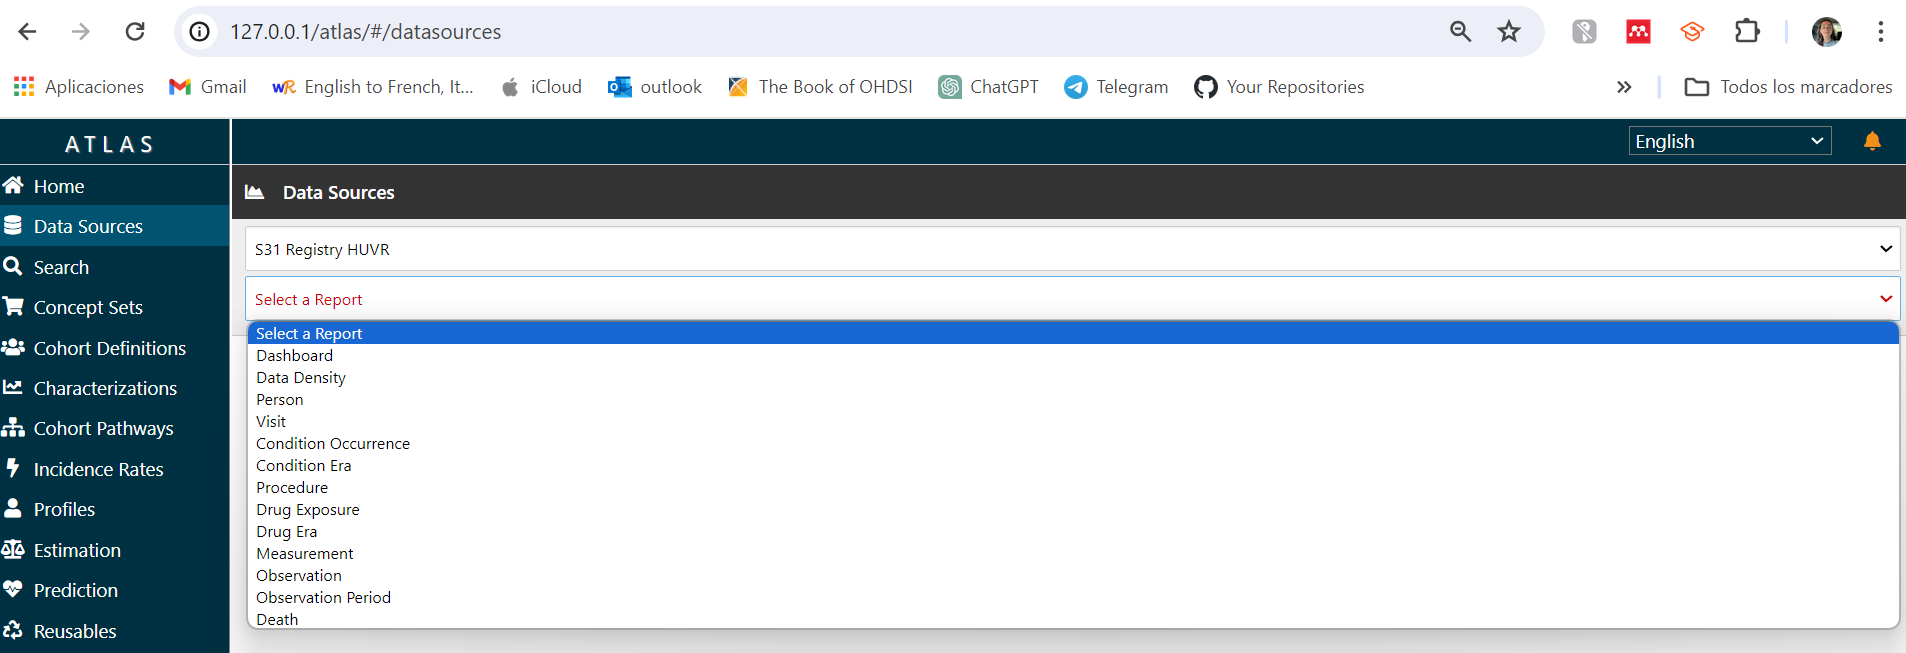
\includegraphics[width=1\textwidth]{figures/atlasDataSources.png}
    \caption{Captura de pantalla de la interfaz principal del menú \code{Data Sources}}
    \label{figure:atlasDataSources}
\end{figure}

A continuación se generan algunos reportes para realizar un análisis exploratorio de la base de datos. Todas las imágenes que se obtienen en cada reporte se encuentran en el repositorio de github \code{Thesis-ATLAS-OHDSI/atlas}.

\begin{figure}[H]
    \centering
    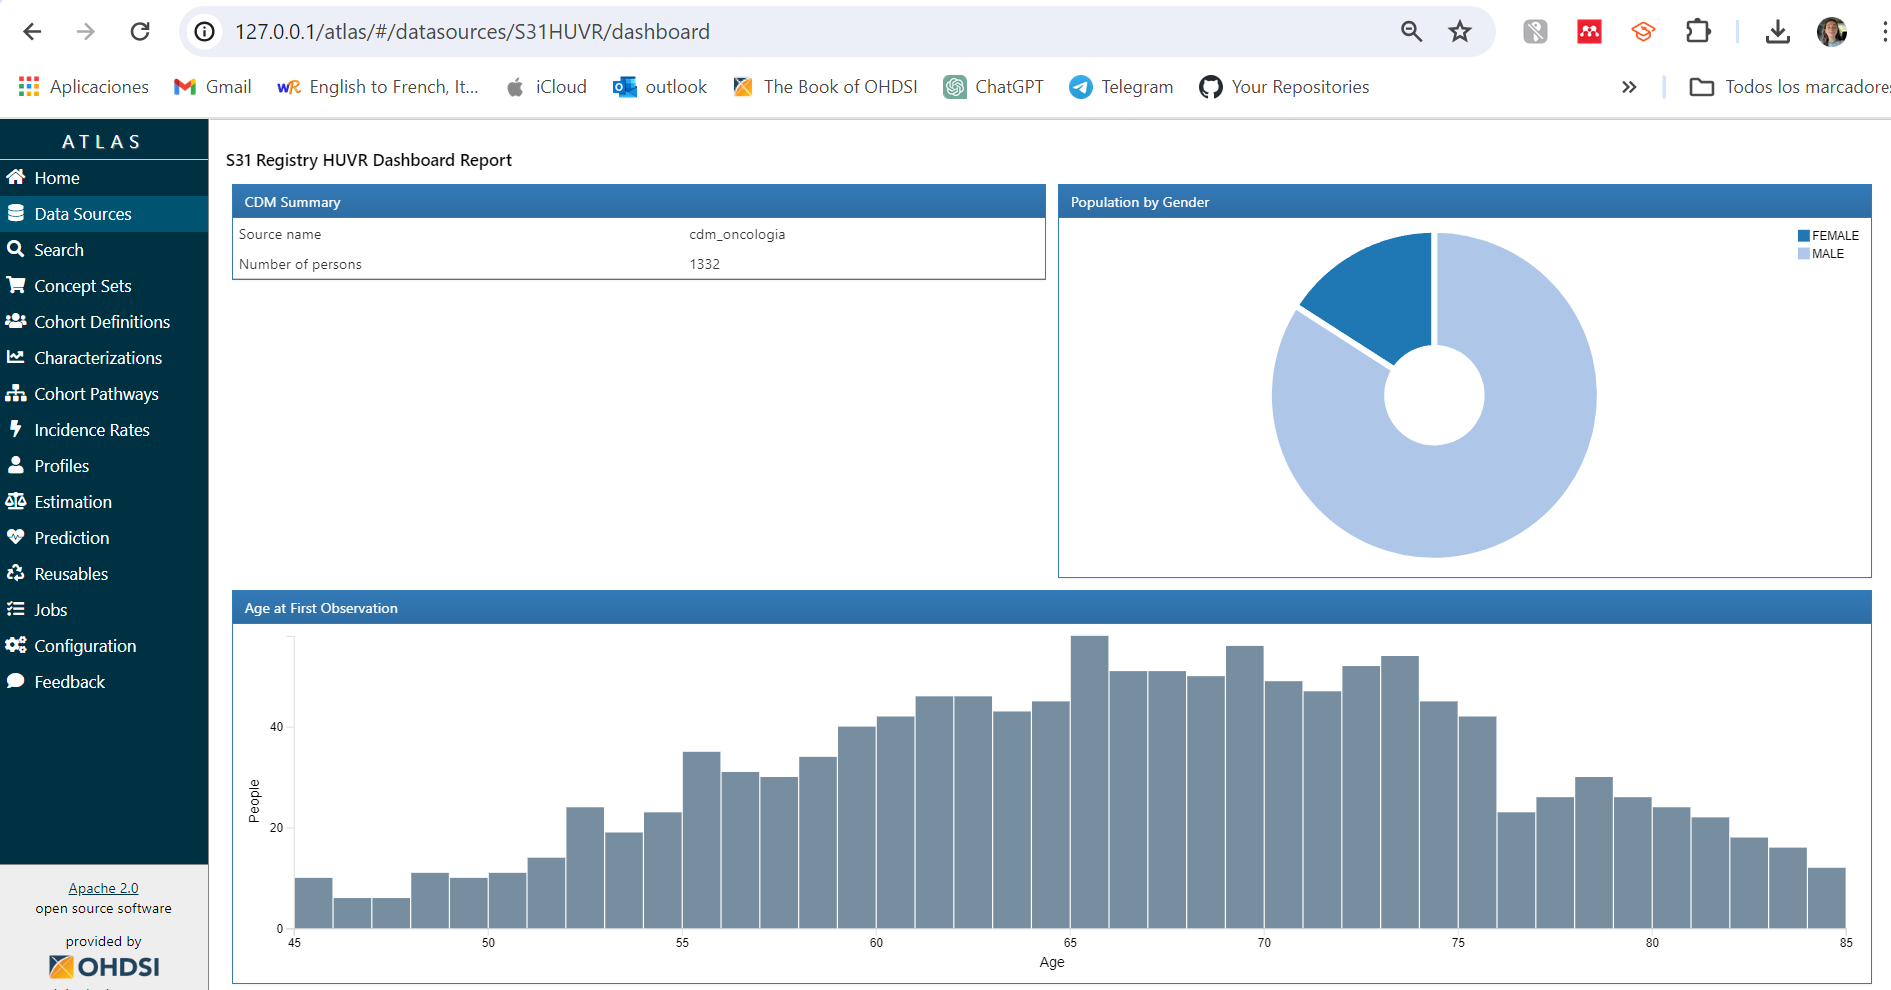
\includegraphics[width=1\textwidth]{figures/atlasCAPdashboard.png}
    \caption{Captura de pantalla del reporte \code{Dashboard} generado en ATLAS Broadsea}
    \label{figure:atlasCAPdashboard}
\end{figure}

\begin{figure}[H]
    \centering
    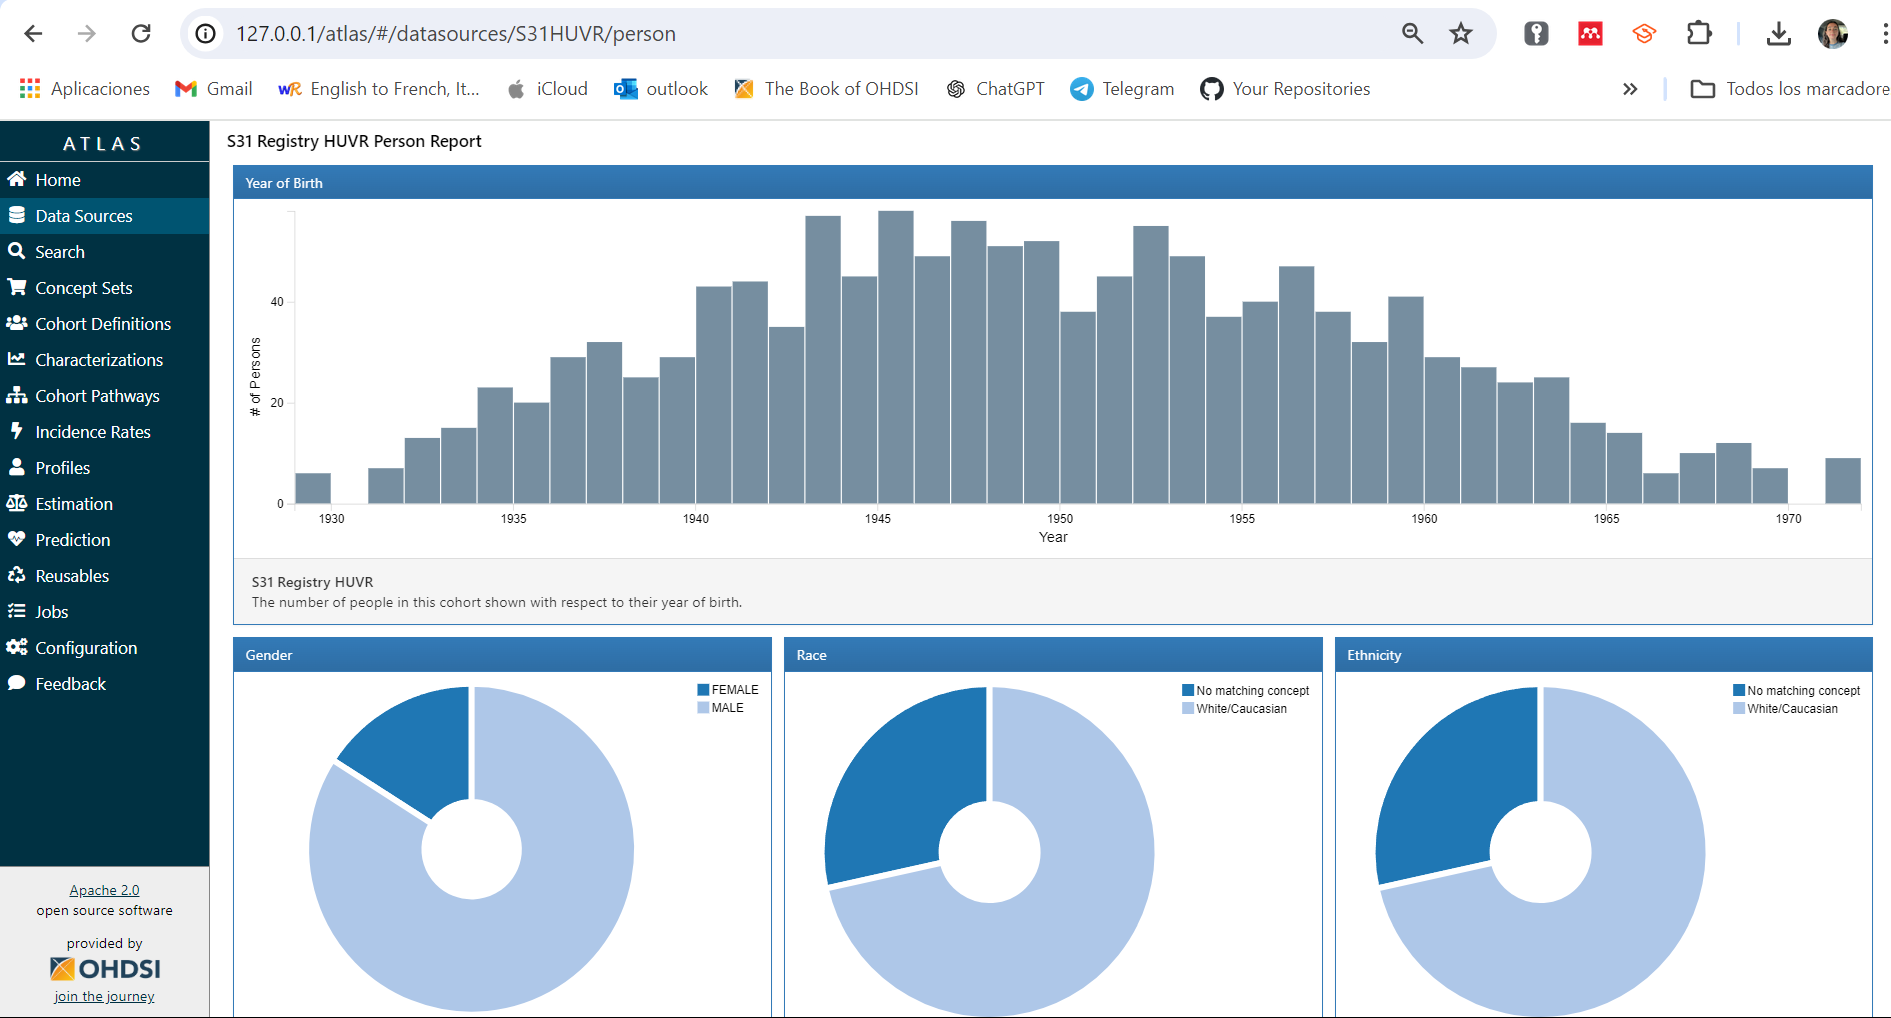
\includegraphics[width=1\textwidth]{figures/atlasREPORTperson.png}
    \caption{Captura de pantalla del reporte \code{Person} generado en ATLAS Broadsea}
    \label{figure:atlasREPORTperson}
\end{figure}

\begin{figure}[H]
    \centering
    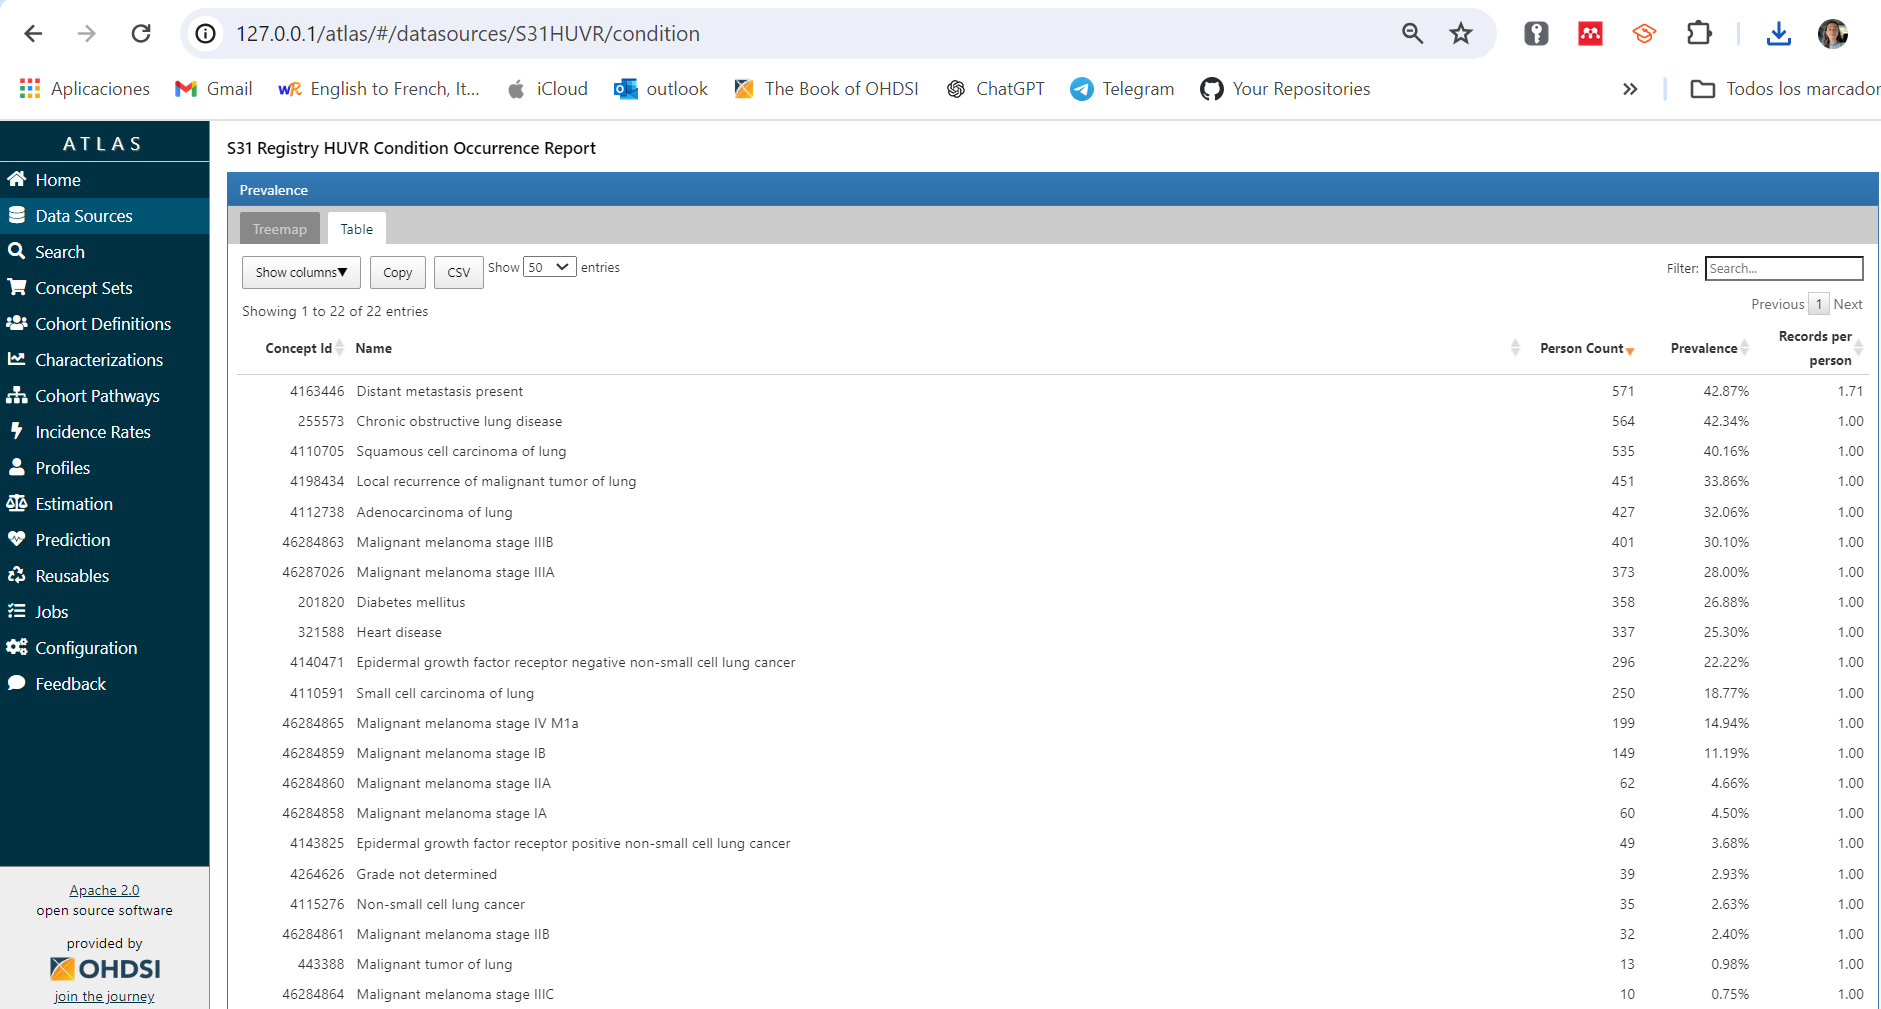
\includegraphics[width=1\textwidth]{figures/atlasREPORTcondition_ocurrence.png}
    \caption{Captura de pantalla del reporte \code{Condition Ocurrence} generado en ATLAS Broadsea}
    \label{figure:atlasREPORTcondition_ocurrence}
\end{figure}

\begin{figure}[H]
    \centering
    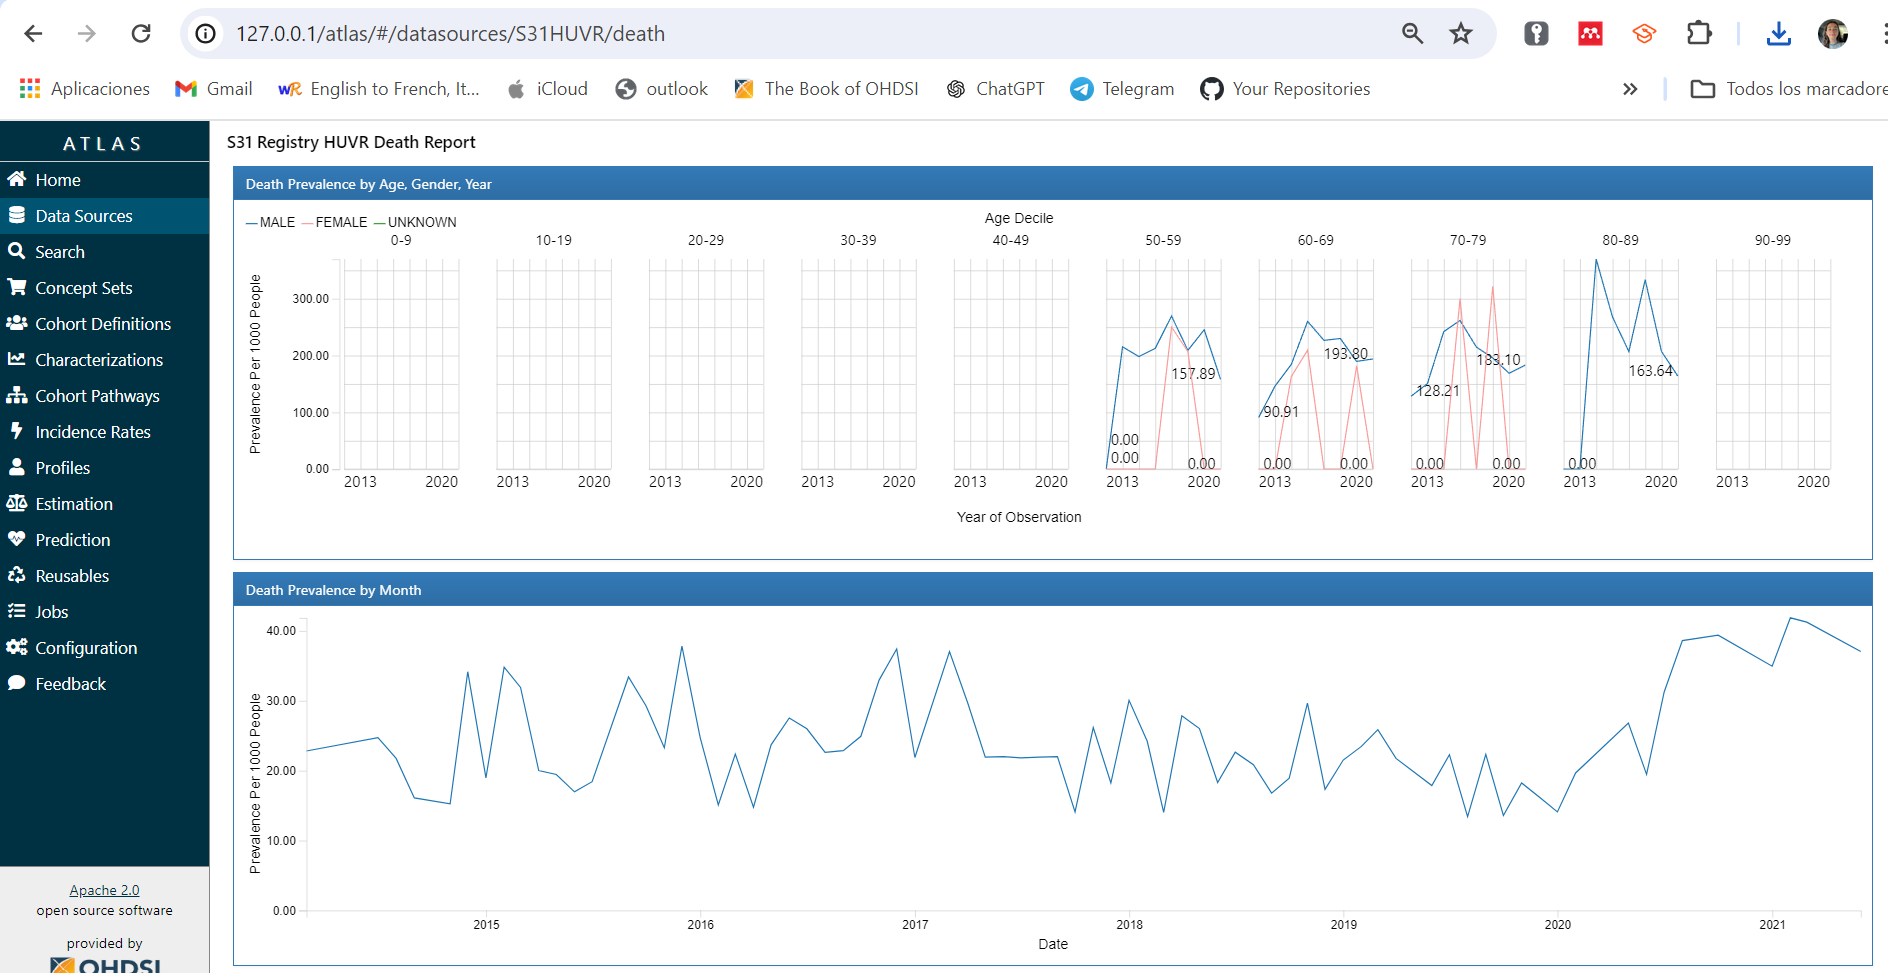
\includegraphics[width=1\textwidth]{figures/atlasREPORTdeath.png}
    \caption{Captura de pantalla del reporte \code{Death} generado en ATLAS Broadsea}
    \label{figure:atlasREPORTdeath}
\end{figure}

\begin{figure}[H]
    \centering
    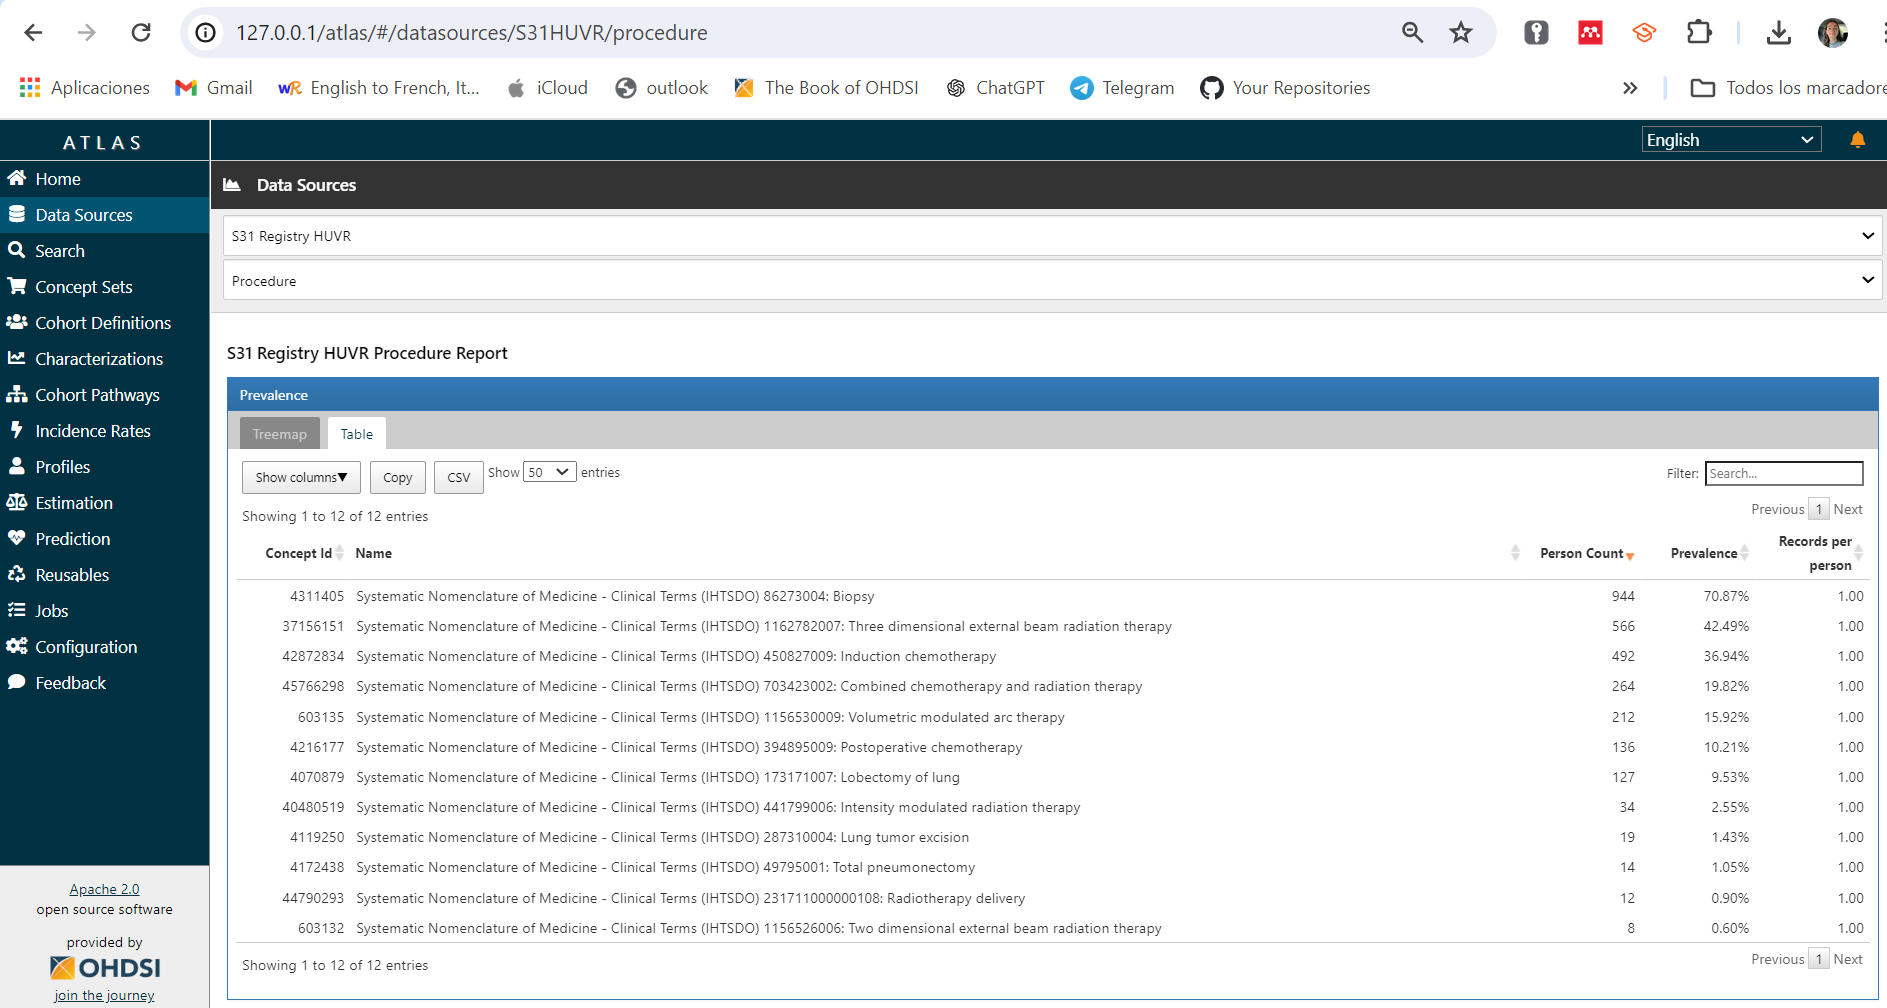
\includegraphics[width=1\textwidth]{figures/atlasREPORTprocedure.png}
    \caption{Captura de pantalla del reporte \code{Procedure} generado en ATLAS Broadsea}
    \label{figure:atlasREPORTprocedure}
\end{figure}

\begin{figure}[H]
    \centering
    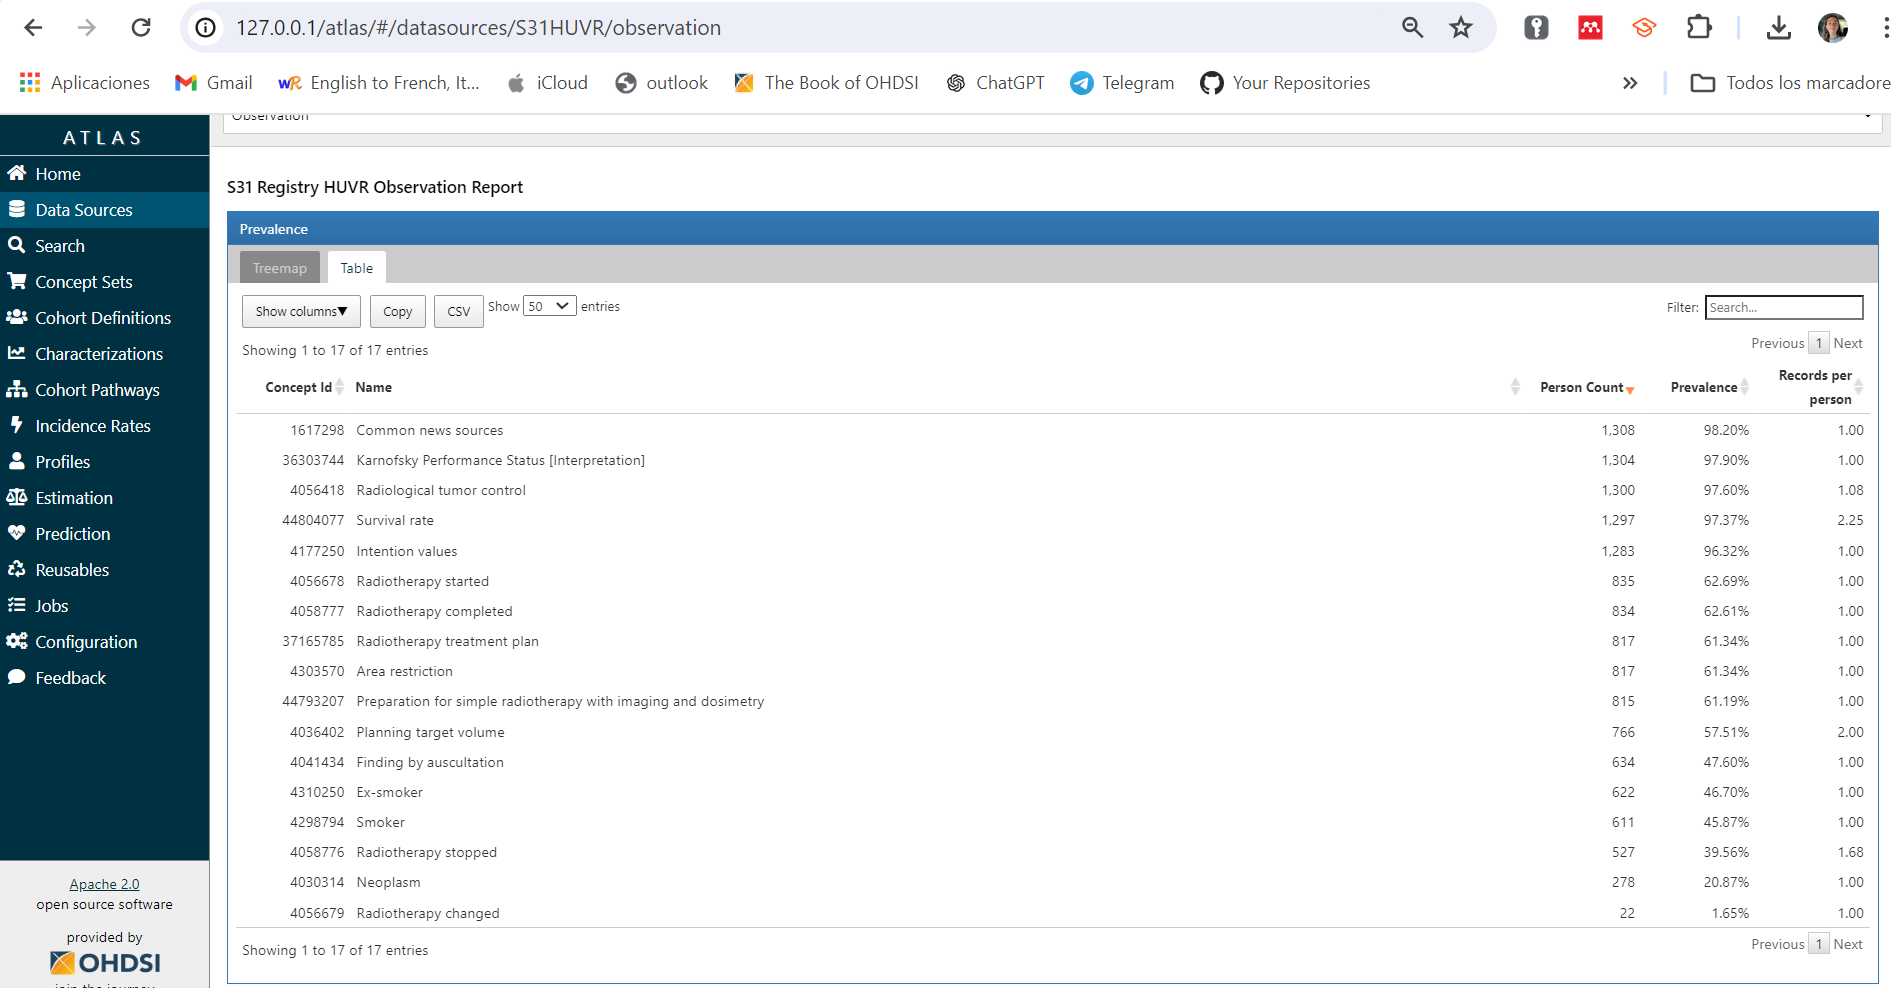
\includegraphics[width=1\textwidth]{figures/atlasREPORTobservation.png}
    \caption{Captura de pantalla del reporte \code{Observation} generado en ATLAS Broadsea}
    \label{figure:atlasREPORTobservation}
\end{figure}